\documentclass{article}
\setlength{\parindent}{0in}
\usepackage[
bottom = 2.50cm,
left   = 2.50cm,
right  = 2.50cm]{geometry}
\newcommand{\code}{\texttt}

\usepackage{graphicx}% Include fig. files
\usepackage{dcolumn}% Align table columns on decimal point
\usepackage{bm}% bold math
\usepackage{caption}
\usepackage[labelformat=simple]{subcaption}
\usepackage{float}
\usepackage{amsmath}
\usepackage{amssymb}
\usepackage[export]{adjustbox}
\usepackage[dvipsnames]{xcolor}
\usepackage{authblk}
\usepackage{url}
\usepackage{listings}
\usepackage{braket}
\usepackage{biblatex}
\addbibresource{ref.bib}

\begin{document}

\title{ESC407 Lab 3}

\author{Maggie Wang}

\date{October 30, 2023}
\maketitle

\begin{enumerate}
\item \textbf{Elliptical orbit of a comet}
\begin{enumerate}
    \item
        The function \code{fit\_ellipse(x, y)} in \code{Lab3\_Q1.py} fits a dataset of ($x$, $y$) coordinates to the general equation of an ellipse,
        \begin{align}
            Ax^2+2Bxy+Cy^2+2Dx+2Fy+G=0,  \label{eqtn:ellipse}
        \end{align}
        by solving the corresponding eigenvalue problem, described as follows.\par
        Equation \ref{eqtn:ellipse} can be written as
        \begin{align*}
            f(a, X) = X\cdot a=0,
        \end{align*}
        where $a=(A,2B,C,2D,2F,G)$ and $X=(x^2, xy, y^2, x, y, 1)$. The parameters of the best fit ellipse are those that minimize the squared distance for each data point $i$,
        \begin{align}
            \delta(a, x) &= \sum_{i=1}^N f(a,X)^2 = a^T(X^TX)a. \label{eqtn:sqrt_dist}
        \end{align}
        To exclude the trivial solution, we impose the constraint $\gamma(a) = B^2-4AC < 0$ on $\delta(a, x)$. The constrained equation can be written as
        \begin{align}
            L(a) &= \delta(a,X)-\lambda(\gamma(a)-\phi)\\
                &= a^T(X^T X)a - \lambda(a^TYa-\phi), \label{eqtn:constrained}
        \end{align}
        where $\phi<0$ and $Y$ is a $(6\times 6)$ constraint matrix such that 
        \begin{align}
            a^TYa &= 4AC-B^2. \label{eqtn:ymtx}
        \end{align}
        To minimize $L$, we solve for where the derivative of $L$ with respect to $a$ is 0. 
        Differentiating Equation \ref{eqtn:constrained} gives us the following eigenvalue problem, where $S=X^TX$,
        \begin{align}
            \frac{1}{\lambda}a &= S^{-1}Y a, \label{eqtn:eigval}
        \end{align}
        which can be solved with \code{np.linalg.eig}.

        Solving for the entries $y_{ij}$ of $Y$ from Equation \ref{eqtn:ymtx}, we find $Y$ has the form of any skew-symmetric matrix $Y'$ plus the sparse matrix $Y_{s}$ where the only non-zero entries are $y_{s, 22}=-1/4$ and $y_{s,31}=4$:
        \begin{align}
            Y &= Y' +   \begin{pmatrix}
                0 & 0 &  & \cdots & & 0
                \\
                0 & -\frac{1}{4} & \ddots & & & 
                \\
                4 & 0 & 0 & \ddots & & \vdots
                \\
                0 & 0 & \ddots & \ddots & \ddots & 
                \\
                \vdots &  & \ddots &\ddots & \ddots  & 0
                \\
                0 &  & \cdots  & 0 & 0 & 0
              \end{pmatrix}.
        \end{align}

        In the implementation of Equation \ref{eqtn:eigval}, $X$ can be written as an $N\times 6$ matrix where each row is the vector $X_i = (x_i^2, x_iy_i, y_i^2, x_i, y_i, 1)$ of the $i^{th}$ data point. For simplicity, we will set all upper diagonal entries of $Y'$ to 1. 
        Thus, we can find the parameters $A$, $B$, $C$, $D$, $F$, $G$ from $a$. 
    \item Figure \ref{fig:1a} shows the best-fit ellipse from the given dataset.
    \begin{figure}[H]
        \centering 
        \captionsetup{margin=3.2cm}
        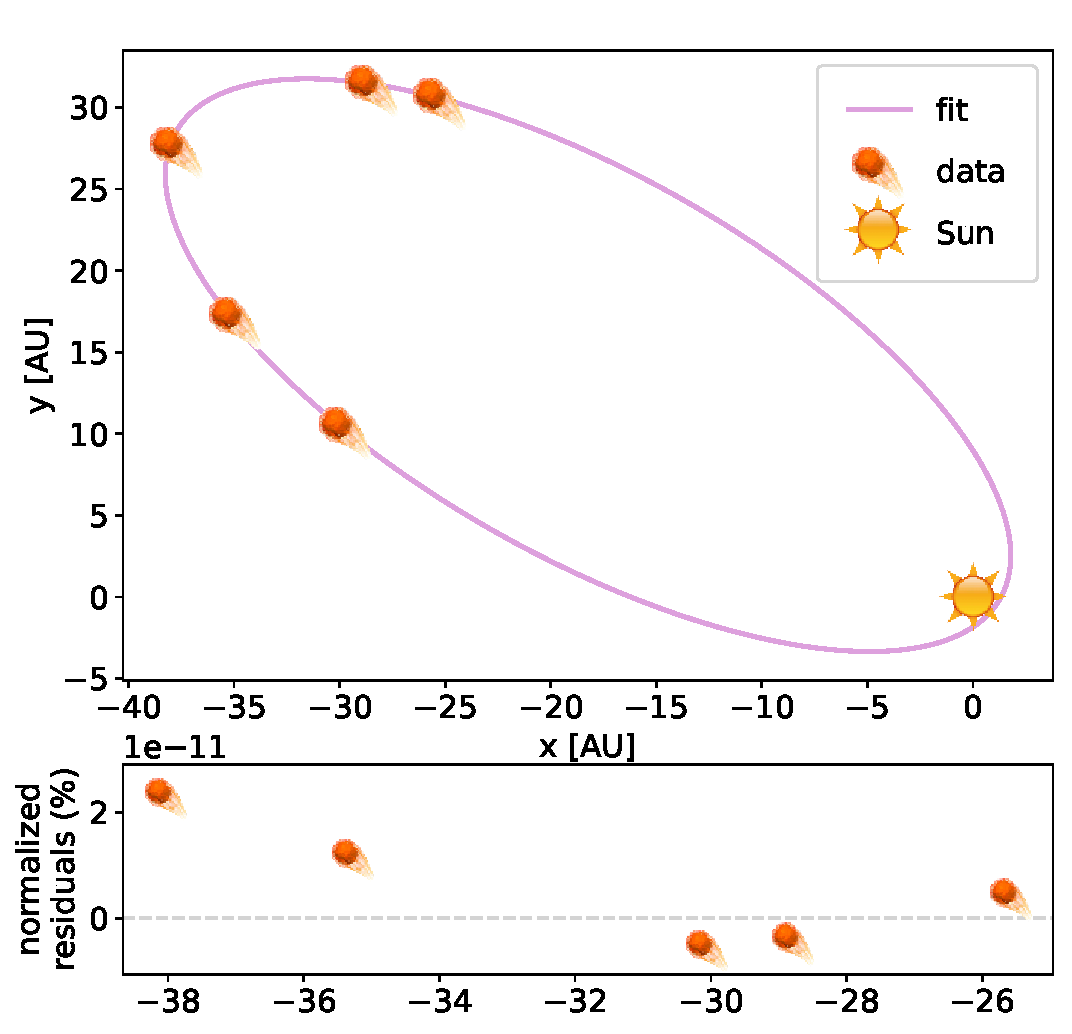
\includegraphics[width=0.5\linewidth]{Q1a.pdf}
        \caption{\label{fig:1a} Best fit ellipse and data points, with $A=-0.0353$, $B=-0.0268$, $C=-0.0460$, $D=-0.2625$, $F=0.1640$, and $G=0.7813$.}
    \end{figure}
\end{enumerate}

\item \textbf{How many computational physicists does it take to screw in a lightbulb?}
\begin{enumerate}
  \item \code{get\_etas(T, l1, l2, lN)} in \code{Lab3\_Q2.py} calculates the efficiency of a perfect blackbody (lightbulb) at temperature T, 
  for radiation between $\lambda_1=$\code{l1} and $\lambda_2=$\code{l2}. The energy radiated between $\lambda_1$ and $\lambda_2$,
  \begin{align}
    E(\lambda_1,\lambda_2) &= \int_{\lambda_1}^{\lambda_2}I(\lambda)d\lambda,
  \end{align}
  is calculated using Gaussian Quadrature with \code{lN} points. The total energy emitted by the lightbulb, $E(0, \infty)$, can be derived analytically when $\lambda_1=0$ and $\lambda_2=\infty$ as 
  \begin{align}
    E(0, \infty) &= \frac{4Ak_b^4\pi^5T^4}{15c^2h^3}.
  \end{align} 
  The area $A$ is a constant factor for all $E$, which drops out of the calculation of $\eta$. For simplicity, we set $A=1$ m$^2$  (and omit it from the code). To determine an appropriate \code{lN}, we compare $E(0,\infty)$ obtained analytically and using Gaussian Quadrature (after applying a change of variables $\lambda=\frac{z}{1-z}$ to the improper integral). 
  \begin{figure}[H]
    \centering 
    \captionsetup{margin=3.2cm}
    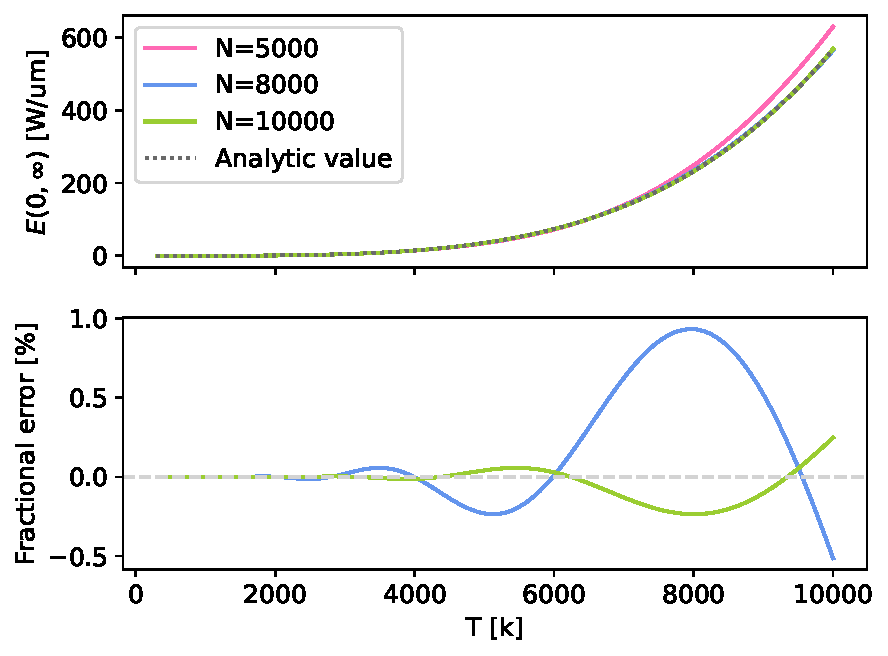
\includegraphics[width=0.48\linewidth]{Q2a.pdf}
    \caption{\label{fig:2a} $E(0,\infty)$ obtained analytically and using Gaussian Quadrature for $A=1$ m$^2$.}
    \end{figure}

  \item Using \code{ln}=10,000, we plot the efficiency $\eta$ from 300 K to 10,000K in Figure \ref{fig:2bd} a). 
  \item Using the golden ratio method to find the temperature of maximum efficiency, we find $T_{max}=6913 K$ and $\eta_{max}=0.49$. Albeit slow, golden ratio suffices in this instance, since the majority of computational power in evaluating $\eta$ arises from finding the weights and positions for Gaussian Quadrature, which only needs to be computed once across all iterations (since the integration bounds are constant)\footnote{To speed up the calculation, we could also take the first derivative of $\eta$ and search for its roots using Newton's method (Binary search is computationally equivalent to Golden Ratio, and it would be hard to isolate for $T$ in $\partial\eta(T)_T$ with which to use the Relaxation method). 
  However, we would then also need to take the second derivative (which has a complicated expression and increases roundoff error due to added operations).}.
  \item For a lightbulb emitting in the infrared, using the same calculation procedure as in a) and c) (with \code{l1}=780 nm and \code{l2}=2250 nm), we find that the temperature of maximum efficiency is now $T_{max}=2925 K$ with $\eta_{max}=0.67$. 
  The IR efficiency from 300 to 10000 K is shown in Figure \ref{fig:2bd} b).
  The temperature of maximum efficiency is impractical for both wavelength ranges, requiring temperatures in the 1000\textdegree Cs. 
  However, the effective temperature of the sun, at 5772 K, is just below the maximum efficiency for emission in the visible wavelength range \footnote{\fullcite{blah}}.
  
  \begin{figure}[h]
    \centering 
    \captionsetup{margin=3.2cm}
    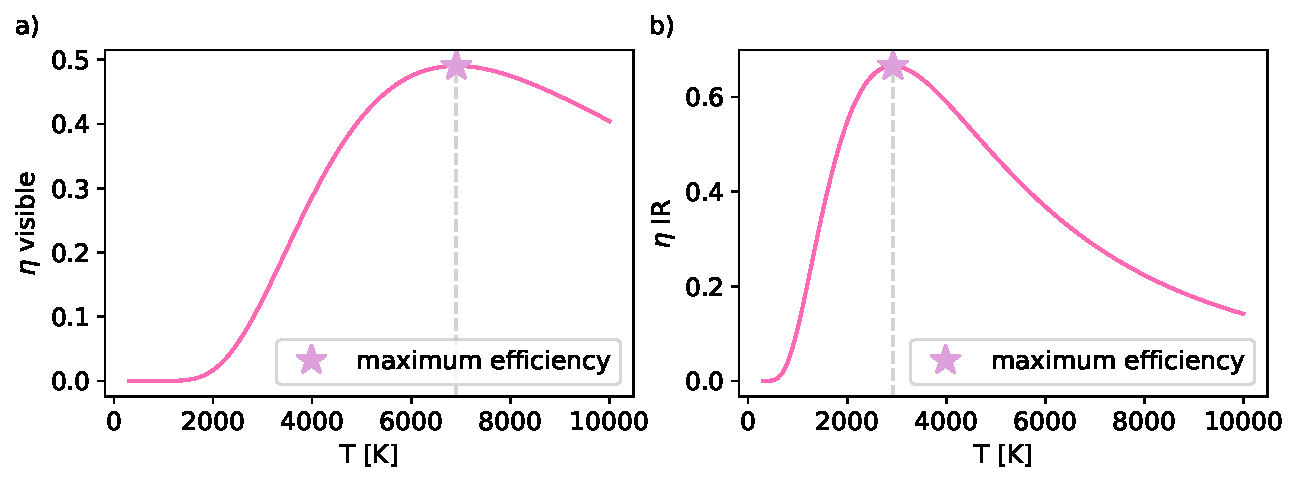
\includegraphics[width=0.8\linewidth]{Q2.pdf}
    \caption{\label{fig:2bd} $\eta$ from 300 K to 10,000K for a) visible (380-780 nm) and b) IR (780-2250 nm) radiation.}
  \end{figure}
\end{enumerate}


\end{enumerate}

\end{document}